
%%%%%%%%%%%   READ COMMENTS IN RED FOR HELP    %%%%%%%%%%%%%%%%%%%%

% For more information use the following link:  https://www.merry.io/courses/learning-latex/

%LaTex dissociates text and equation symbols. To write equations refer to the following link: https://en.wikibooks.org/wiki/LaTeX/Mathematics

% The documentclass determines the type of document you are going to write
\documentclass[ a4paper, 12pt, oneside ]{article} %A4 layout, font 12 points, text is in one column

% Math packages to do equations, tables and figures
\usepackage{mathptmx}
\usepackage{amssymb}
\usepackage{amsmath}
\usepackage{amsfonts}
\usepackage{amsbsy}
\usepackage{graphicx}
\usepackage{tabularx}
\usepackage[svgnames]{xcolor} % Enabling colors by their 'svgnames'

% Language
\usepackage[english]{babel} 
\usepackage{mathpazo} % Palatino font

% Figure captions
\usepackage[font={small,it}]{caption}

% enumeration
\usepackage{enumerate}

% Depth of the table of contents
\setcounter{tocdepth}{2}

% footnotes at the bottom of the page
\usepackage[bottom]{footmisc} 

%%%%%%%%% PAGES %%%%%%%%%%%%%%
\usepackage{fancyhdr}
\pagestyle{fancy}
\fancyhf{}
\fancyhead[LE,RO]{NAME OF THE PROJECT}
\fancyhead[RE,LO]{Final Report}
\fancyfoot[CE,CO]{\leftmark}
\fancyfoot[LE,RO]{\thepage}

\renewcommand{\headrulewidth}{2pt}
\renewcommand{\footrulewidth}{1pt}

% Begin the document
\begin{document} %The document begins here

% If this is an BEng project.
%%%%%%%%%%%%%%%%%%%%%%%%%%%%%%% TITLE SETTINGS %%%%%%%%%%%%%%%%%%%%%%%%%%%%%%%%%%%%%%%%%%%%%%%%%%%%%%%%%


%----------------------------------------------------------------------------------------
%	TITLE PAGE
%----------------------------------------------------------------------------------------

\begin{titlepage} % Suppresses displaying the page number on the title page and the subsequent page counts as page 1

%%%%%%%%%%%%%%%%% TO INCLUDE A BANNER %%%%%%%%%%%%%%%%%%
% To include your banner remove the % for the next four lines and include in \includegraphics the name of the file

\begin{figure}[!htb]
\centering

\includegraphics[width=\linewidth]{Banner1.eps}
\end{figure}

%%%%%%%%%%%%%%%%%%%%%%%%%%%%%%%%%%%%%%%%%%%%%%%%%


	\newcommand{\HRule}{\rule{\linewidth}{0.5mm}} % Defines a new command for horizontal lines, change thickness here
	
	\center % Centre everything on the page
	
	%------------------------------------------------
	%	Headings
	%------------------------------------------------
	
	\textsc{\LARGE University College London (UCL)}\\[1.5cm] % Main heading such as the name of your university/college
	
	\textsc{\Large ELEC0036}\\[0.5cm] % Major heading such as course name
	
	%\textsc{\large  Report}\\[0.5cm] % Minor heading such as course title
	
	%------------------------------------------------
	%	Title
	%------------------------------------------------
	
	\HRule\\[0.4cm]
	
	{\huge\bfseries TITLE}\\[0.4cm] % Title of your document
	
	\HRule\\[1.5cm]
	
	%------------------------------------------------
	%	Author(s)
	%------------------------------------------------
	
	\begin{minipage}{0.4\textwidth}
		\begin{flushleft}
			\large
			\textit{Author}\\
			FIRST NAME \textsc{LAST NAME} % Your name
		\end{flushleft}
		  \hfill		
	\end{minipage}
         ~
	\begin{minipage}{0.4\textwidth}
		\begin{flushright}
			\large
			\textit{Student Number}\\
			 \textsc{number} % Your student number
		\end{flushright}
	\end{minipage}
	~
	\begin{minipage}{0.4\textwidth}
		\begin{flushleft}
			\large
			\textit{Supervisor}\\
			Dr./ Prof \textsc{LAST NAME} % Supervisor's name
		\end{flushleft}
	\end{minipage}
	~
	\begin{minipage}{0.4\textwidth}
		\begin{flushright}
			\large
			\textit{Second Supervisor}\\
			Dr./Prof  \textsc{LAST NAME} % Supervisor's name
		\end{flushright}
	\end{minipage}
	% If you don't want a supervisor, uncomment the two lines below and comment the code above
	%{\large\textit{Author}}\\
	%John \textsc{Smith} % Your name
	
	%------------------------------------------------
	%	Date
	%------------------------------------------------
	
	\vfill\vfill\vfill % Position the date 3/4 down the remaining page
	
	{\large\today} \\% Date, change the \today to a set date if you want to be precise
	{\large \textbf{A BEng Project Final Proposal}}
	%------------------------------------------------
	%	Logo
	%------------------------------------------------
	
	%\vfill\vfill
	%\includegraphics[width=0.2\textwidth]{banner.pdf}\\[1cm] % Include a department/university logo - this will require the graphicx package
	 
	%----------------------------------------------------------------------------------------
	
	\vfill % Push the date up 1/4 of the remaining page
	
\end{titlepage}

%----------------------------------------------------------------------------------------
 % This command includes whatever is in the document title_settings.tex

% Start the Table of Contents on a new page
\newpage %create a new page

\tableofcontents %Add a table of content

\newpage

%%%%% Abstract
\abstract{This is the most important paragraph in the entire proposal. It is a snapshot of the proposed work. It is a concise summary of what is intended to be accomplished and gives a short indication of what has appeared in the literature before you start your work. Keep it about 300 words (under one page). The Abstract is written last, after the entire proposal has been written. Use the funnel approach: Make a general statement about the topic; then say something about what is missing from the past and current research or current theory or whatever (his is a very brief historical review in just a couple of sentences); let the reader know what you intend to do to fix that; lastly, indicate your major result(s).

% Write your abstract here between the brackets
% Summarise your objectives
% Summarise your Approach here
% Summarise your main result here
% Summarise the significance of your results here

%%%%% Sections
\section{Introduction} %Section creates sections starting from 1
\label{introduction} %You can refer to a label anywhere in the text and the reader will be directed to the label, no matter how the paper changes.
Think of the introduction as a development of the context for the reader. Peruse the literature quickly. Highlight the historical progression of the theory and work that has been done, citing the literature as you go. Use the citation mechanisms in the editor you are using. If it is Word, you can use its bibliographic reference tool or Mendeley or another third-party add-on. Use IEEE citing format. After the reader has some idea of what the historical background is, mention what is missing in it that your proposal is going to fill

If you would like to cite something, write this: \cite{ELEC0036_PP_2020}. It has to be in the bibliography. See below. To compile it, you need to compile first the LaTex file, then switch the compiler to BibTex or whatever your reference compiler is and compile, then compile the LaTex file again twice to catch everything.

Here are some hints and ideas for a better paper:
\begin{enumerate}
\item{ Writing Hints:
\verb*|\emph{}| emphasises the word in brackets}
% \underline{} underlines the word in the brackets
% textbf{} for a bold font
% To include symbols such as & and % write them as follow: \% and \&

\item{ Figures:
To add a figure use the following lines by including the file name in includegraphics 
Give a reference name inside \label{} brackets so you can refer automatically to the figure's number by using the function \verb*|\ref{name}|. You can use the same functions to refer to a section, using \verb*|\label{name}| to label something.

\begin{verbatim}
\begin{figure}[H] 
\centering
\includegraphics[width=\textwidth]{name of the file} 
\caption{title of the figure}
\label{give a reference name}
\end{figure}
\end{verbatim}
}

\item{Subsections: 
\verb*|\subsection{title}| creates a sub-section such as 1.1 and \verb*|\subsubsection{title}| creates a sub-sub-section such as 1.1.1. For more subsections use the command \verb*|\paragraph{title}|. }
\item{To cite a reference use the function \begin{verbatim}\cite{Yonge_1856}\end{verbatim} It appears within the text like this: \cite{Yonge_1856} and you will see it in the references later. You need to use a reference management software package such as BibDesk. See the bibliography note below.}

\item{If at any point for some reason your document is not compiling, remove the following file: nameOfPaper.aux}

\item{ Compiling and Layout: When you want to see your references, first compile the reference document (.tex file) using the first item in the popup list in the upper left hand corner of the .text window. You might want to compile it twice to be sure the references are all caught. Then compile the bibtex document (.bib file) using the second item in the popup list of the .tex window. Then compile the LaTex File again. You may also want to compile it several times to avoid any problems such as missing content in the table of contents.}

\item{ You can find more templates at the following link: \\
https://www.latextemplates.com/}
\end{enumerate}

\section{Goals and Objectives} \label{goals}
Your objectives are the most important part of the proposal. Tell the reader what you intend to accomplish; see if you can state the expected outcomes in a clear fashion so that you know, and the reader knows, what you are going to have when finished. What theory will you work out? Or what measurements will you make? Or what circuit will you build? The clearer you are with this, the higher the chances will be for knowing how to get there.
Break the Objectives down into pieces on which each of your teammates will focus. Show how the individual objectives create the project?s overall end objective.
 6/7
 Once you know what you will be doing, put the steps into a Gantt Chart. Look online for a Gantt Chart description if you need to. Your chart may look like that in fig. \ref{Fig:GanttChart}. Use the Figure environment to insert it (see above).

\begin{figure}[h] 
\centering
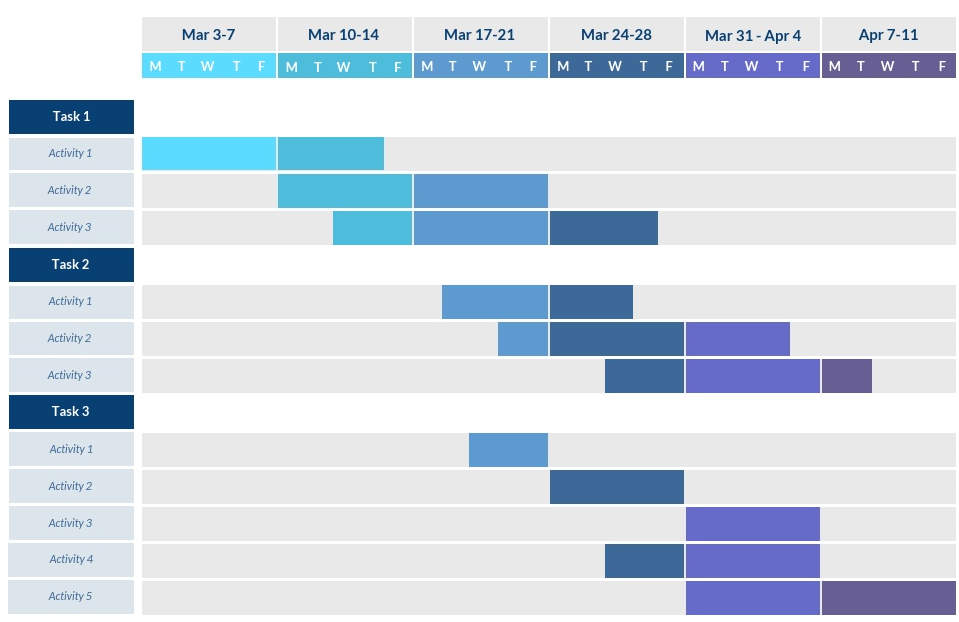
\includegraphics[width=\textwidth]{SampleGanttChart.png} 
\caption{This is a sample Gantt Chart. You can find out how to make one on-line.}
\label{Fig:GanttChart}
\end{figure} 
 
 % Write here your text

\section{Preliminary Assessment of Risks} 
\label{sec:RiskAssessment}
\begin{itemize}
\item{\textbf{Safety Risks}: Please identify the Laboratories in which you will work. The Managers of these labs MUST approve the assessment forms you have filled in. If you can, try to meet with them and show them the assessments you are planning to post. The forms are available on Moodle.

\textbf{You will not be allowed to start working in any laboratory until your assessment of safety risks is approved by the lab manager.}}

\item{\textbf{Failure Risks}: These are your estimates of the risks you face with your current plan. If you indicate a high risk of failure, that is, something with which you are uncomfortable, you should outline a new plan to use as backup in case the current plan does not work out for you. You can record the details of any alternative plan in your December Interim Report.}
\end{itemize}

\newpage
Your Bibliography should appear on this page, if you use BibTex. For example:
\bibliographystyle{ieeetran} %style of the bibliography. You can look for other styles online
\bibliography{project_proposal_template} %prints the bibliography by writing its name in the brackets

% For IOS, download BibDesk from the following link: https://bibdesk.sourceforge.io/

%For Windows, Mac or Linux download Mendeley from the following link: https://www.mendeley.com/download-desktop-new?mboxSession=455e210fe7164ae5be72907cf43d80b0&adobe_mc_sdid=SDID%3D1771E6E0BD7935A0-1E92E999E8893227%7CMCORGID%3D4D6368F454EC41940A4C98A6%40AdobeOrg%7CTS%3D1583323671&adobe_mc_ref=https%3A%2F%2Fwww.google.com%2F

%For Windows, Mac or Linux download JabRef from the following link: https://www.jabref.org/

\end{document}















